
\section{Modellbildung}
\begin{tabularx}{\columnwidth}{p{2.8cm}XX}
	\hline 
	\multicolumn{3}{c}{\textbf{Grundbegriffe}}\\
	Diffgleichung n-ter Ordnung & $F(x,y,y',y'',\dots, y^{(n)}) = 0$ & 
	Intervall: $I\subseteq R$ \newline 
	Bereich: $\Omega \subseteq I \times \mathbb{R}^{n+1}$ \newline stetige Funktion $F: \Omega \rightarrow \mathbb{R}$ \\
	\hline 
	explizite  DGL &$y^{(n)} = G(x,y,y',y'',\dots,y^{(n-1)}$ & nach $y^{(n)}$ aufgelöst\\
	implizite DGL & nicht nach $y^{(n)}$ aufgelöst & \\
	\hline 
	Lösung von DGL & n mal differenzierbare Funktion &$\forall x\in I$ \\
	
	 & Lösen einer DGL gibt eine allgemeine Lösung & Lösen eines Anfangswertproblems/Randewrtproblems ergibt  spezielle, partikuläre Lösung\\
	Anfangswertproblem & $\begin{cases}
		F(x,y,y',y'',\dots, y^{(n)}) & = 0,\quad  (x,y,\dots,y^{n}) \in \Omega \\
		y(x_0)  &= y_0\\
		y'(x_0) &= y_1\\
				&\vdots \\
						y^{n-1}(x_0) &= y_{n-1}\\
	\end{cases}$& 
	\\
	Randwertprobleme & \multicolumn{2}{p{14cm}}{andere Phänomene als bei Angfangswertproblemen, Existenz- und Eindeutigkeitsaussagen für AWPs nicht mehr}\\
	\hline 
	\multicolumn{3}{c}{\textbf{Klassifikation}}\\
	linear & $a_n(x)\cdot y'(n) + \cdots + a_1(x)\cdot y' + a_0(x)\cdot y = g(x)$ & $a_i(x)$: fest vorgegebene funktionen\\
	homogen & $g(x) = 0 \quad \forall x\in I$ & $g(x)$: Störfunktion, Ihomogenität \\
	konstante Koeffizienten & $a_n\cdot y'(n) + \dots + a_1\cdot y' + a_0\cdot y = g(x)$  & $a_i$: konstante Koeffizienten, $a_n\neq 0$\\
	\multicolumn{3}{c}{spezialfälle 1. Ordnung}\\
	linear & $y' = f(x)\cdot y + g(x) $ & \\
	Exakte DGL & $M(x,y) + N(x,y)\cdot y'(x) = 0$ & Bedingung: $M_y(x,y) = N_x(x,y)$\\
	separierbar & $y' = g(x)\cdot h(y)$ & \\
	autonom & $y' = f(y)$ & autonom $\subseteq$ separierbar, $ g(x) = 1$  \\
	Typ unbestimmtes Integral & $y' = g(x)$ & separierbar aber nicht autonom\\
	\hline 
	\multicolumn{3}{c}{\textbf{Systeme von Differentialgleichungen}}\\
	
	System von DGL 1. Ordnung & 
	\multicolumn{2}{p{14cm}}{ $\begin{matrix} y_1' &=& f_1(x,y_1,\dots,y_n) \\ \vdots & &\vdots \\ y_n' &=& f_n(x,y_1,\dots,y_n)\\\end{matrix} \qquad $ 
	$\bm{y}(x) = \left(\begin{matrix} y_1(x) \\ \vdots \\ y_n(x)\end{matrix} \right) , \quad
	\bm{f}(x, \bm y) = \left(\begin{matrix} f_1(x,\bm y) \\ \vdots \\ f_n(x, \bm y)\end{matrix} \right)$}\\
	vektorielle Schreibweise & $\bm y' = \bm f(x,\bm y)$ & \\
	
	Anfangswertproblem & $\begin{cases} \bm y' & = \bm f(x,\bm y),\quad (x,\bm y)\in \Omega\subseteq \mathbb{R}\times\mathbb{R}^n \\ \bm y(x_0) &= \bm y_0\end{cases}$ & \\
	\hline
	\multicolumn{3}{c}{\textbf{Richtungsfeld}}\\
	$y'=F(x,y)$&
	DGL ,$n=1$, explizit: jedem Punkt $(x,y)$ wird ein Steigungswert zugeordnet ergibt Richtungsfeld & 
	 \raisebox{-.8\totalheight}{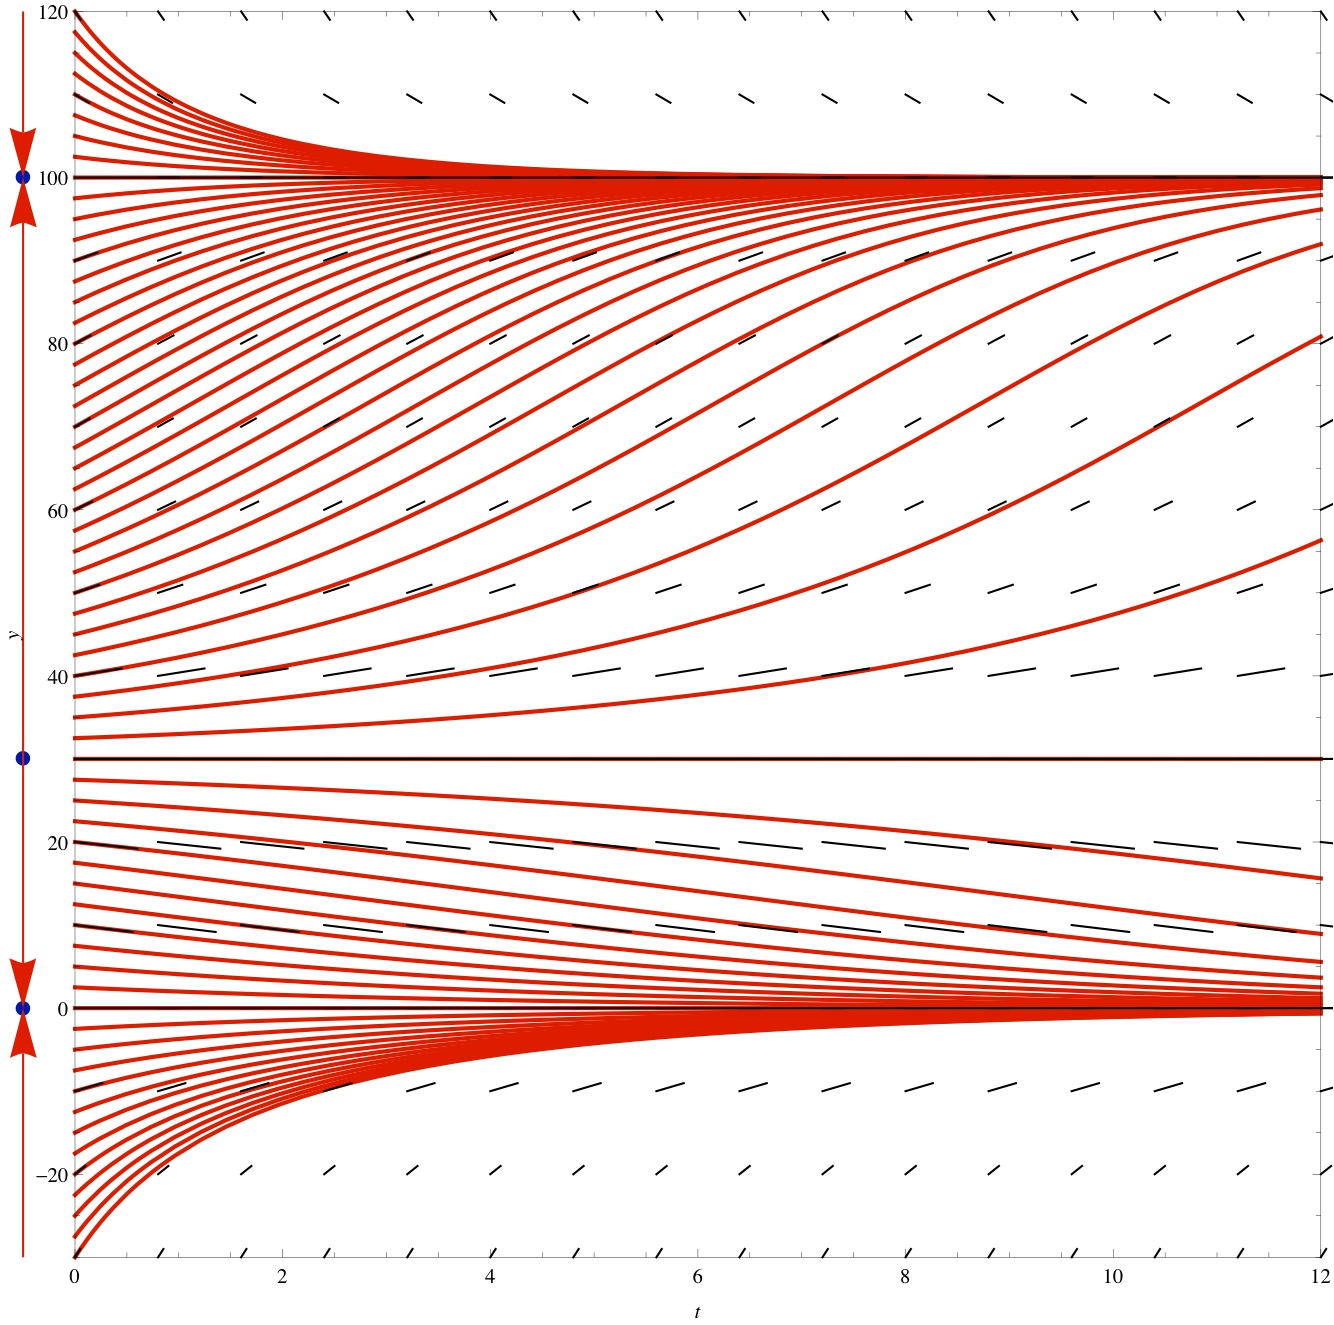
\includegraphics[scale = .15]{images/richtungsfelder}}\\
	Typ unbestimmtes Integral & Richtungsfeld y- unabhängig & \\
	autonome DGL & Richtungsfeld x-unabhängig & \\
	\hline 
	\multicolumn{3}{c}{\textbf{Lösbarkeit}}\\
	Lipschitz-Stetigkeit & $|\bm f(x,\bm y_1) - f(x,\bm y_1)| \leq L|\bm y_1 - \bm y_2|$ & $f(x,\bm y)$ muss stetig sein und Libschitz-Stetigkeit erfüllen für Eindeutigkeit\\
	Erüfllt wenn & 	 $\dfrac{\partial \bm f(x,\bm y_i)}{\partial y_i}$ stetig ist & \\
	Piccard-Lindelöf &\multicolumn{2}{p{14cm}}{ offene Menge: $\Omega \subseteq \mathbb{R}\times \mathbb{R}^n $\newline
	zulässige Funktion$ \bm f:\Omega \rightarrow\mathbb{R}^n \quad (x,\bm y) \mapsto \bm f(x,\bm y)$\newline 
	beliebiger Punkt $  (x_0,\bm y_0)\in \Omega$ \newline 
	$\rho > 0$ hinreichend klein $\bm y(x): [x_0-\rho,x_0+\rho] \to \mathbb{R}^n \Rightarrow$ \newline 
	dann existiert genau eine Lösung }\\
\end{tabularx}
